%=========================================================================
% Start of activity on angle sum formulae
%=========================================================================
\preClass{Distance Between Two Points}

\begin{problem}
\item Determine the distance between the points $P$ and $Q$ using the distance formula.
  \sideNote{Write out the expression, FOIL out the squared terms, and simplify as much as possible.}

  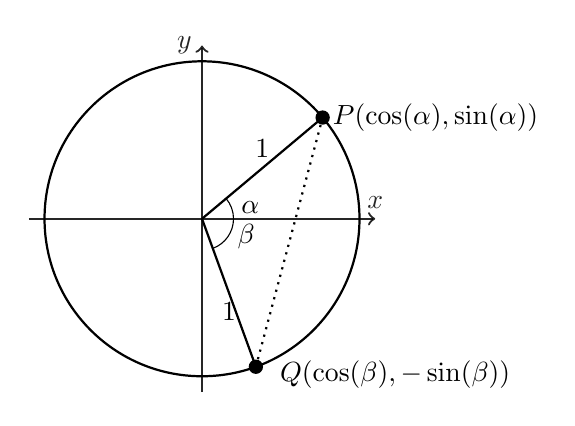
\begin{tikzpicture}[y=2cm, x=2cm,font=\sffamily]
      \draw[thick,opacity=0.85,->] (0, -1.1) -- (0,1.1) node[anchor=east] {$y$};
      \draw[thick,opacity=0.85,->] (-1.1, 0) -- (1.1,0) node[anchor=south] {$x$};
      \draw[thick] (1,0) arc (0:360:1);
      \draw[thick] (0,0) -- (40:1) node[midway,anchor=south] {$1$}
          node[anchor=west] {$P(\cos(\alpha),\sin(\alpha))$};
      \draw[text=black] (0:0.2) arc (0:40:0.2) node[midway,anchor=west] {$\alpha$};
      \fill[black] (40:1) circle [radius=0.6ex]; % Draw a dot
      \draw[thick] (0,0) -- (-70:1) node[midway,anchor=north] {$1$}
          node[anchor=west,xshift=5,yshift=-3] {$Q(\cos(\beta),-\sin(\beta))$};
      \draw[text=black] (0:0.2) arc (0:-70:0.2) node[midway,anchor=west] {$\beta$};
      \fill[black] (-70:1) circle [radius=0.6ex]; % Draw a dot
      \draw[black,thick,dotted] (40:1) -- (-70:1);
    \end{tikzpicture}

    \vfill

\item Determine the distance between the points $R$ and $S$ using the distance formula.
  \sideNote{Write out the expression, FOIL out the squared terms, and simplify as much as possible.}

  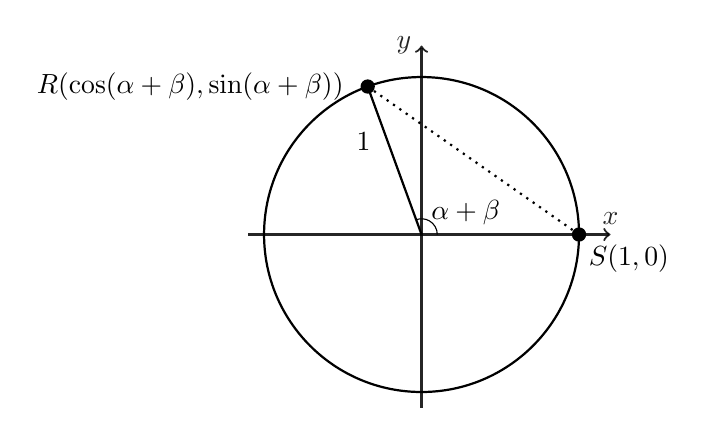
\begin{tikzpicture}[y=2cm, x=2cm,font=\sffamily]
      \draw[thick,opacity=0.85,->] (0, -1.1) -- (0,1.2) node[anchor=east] {$y$};
      \draw[thick,opacity=0.85,->] (-1.1, 0) -- (1.2,0) node[anchor=south] {$x$};
      \draw[thick] (1,0) arc (0:360:1);
      \draw[thick] (0,0) -- (110:1) node[midway,anchor=south east,xshift=-5] {$1$}
          node[anchor=east,xshift=-5] {$R(\cos(\alpha+\beta),\sin(\alpha+\beta))$};
      \draw[text=black] (0:0.1) arc (0:110:0.1);
      \node[midway,anchor=south west,xshift=0] at (45,0.2) {$\alpha+\beta$};
      \fill[black] (110:1) circle [radius=0.6ex]; % Draw a dot
      \fill[black] (1,0) circle [radius=0.6ex] node[anchor=north west] {$S(1,0)$};
      \draw[black,thick,dotted] (110:1) -- (1,0);
    \end{tikzpicture}

    \vfill

  \item What is the relationship between the two distances? 
    
    
\end{problem}


\actTitle{Angle Sum Formulas}
\begin{problem}
\item Determine the exact values of each of the following expressions
  without using any trigonometric functions.
  \begin{subproblem}
  \item ${\displaystyle \cos(\arctan(0.1)+\arccos(-0.8))}$
    \vfill
  \item ${\displaystyle \sin(\arcsin(-0.4)+\arctan(0.6))}$
    \vfill
  \item ${\displaystyle \sin(\arccos(-0.4)+\arcsin(0.6))}$
    \vfill
  \end{subproblem}

  \clearpage

\item Show that the following expressions are identities.
  \begin{subproblem}
  \item ${\displaystyle \sin(2\theta)=2\sin(\theta)\cos(\theta)}$.
    \vfill
  \item ${\displaystyle \cos(2\theta)=\cos^2(\theta)-\sin^2(\theta)}$.
    \vfill
  \end{subproblem}

  \clearpage

\item Use the double angle formulas to expand the expression
  \begin{eqnarray*}
    \cos(\alpha+\beta) + \cos(\alpha-\beta).
  \end{eqnarray*}
  Simplify the expression as much as possible.  Make up an expression
  involving the sine function that will reduce in a similar way.

  \vfill

  \clearpage

\item Using the two identities
  \begin{eqnarray*}
    \sin(2\theta) & = & 2\sin(\theta)\cos(\theta), \\
    \cos(2\theta) & = & \cos^2(\theta)-\sin^2(\theta),
  \end{eqnarray*}
  use what you know about the values of $\cos\left(\frac{\pi}{6}\right)$ and
    $\sin\left(\frac{\pi}{6}\right)$ to determine the values of
      $\cos\left(\frac{\pi}{12}\right)$ and $\sin\left(\frac{\pi}{12}\right)$.

  \vfill
  
\end{problem}

\postClass

\begin{problem}
\item Briefly state two ideas from today's class.
  \begin{itemize}
  \item 
  \item 
  \end{itemize}
\item 
  \begin{subproblem}
    \item
  \end{subproblem}
\end{problem}


%%% Local Variables:
%%% mode: latex
%%% TeX-master: "../labManual"
%%% End:

